\section{Misura della lunghezza d'onda di una lampada a mercurio}
\subsection{Calibrazione}
In questa fase si cerca di porre in relazione la differenza 
di cammino ottico $\Delta x$ allo spostamento letto 
sul micrometro $\Delta L$,
ovvero il fattore di demoltiplica della leva $y$.
Per effettuare tale calibrazione abbiamo 
montato una sorgente di  $\lambda$ nota, nello specifico un laser
He-Ne di $\lambda=\unit{632.8}{\nano\meter}$.
Posta la scala del micrometro, in corrispondenza dello zero,
attraverso il meccanismo posto su M2 si sono allineati i fasci 
uscenti dai de bracci dell'interferometro;
dopodiché si è preso 
come riferimento un punto e si sono contate il numero di frange che si vedono 
passare al variare di $\Delta L$.
Essendo valida \smallskip
\begin{equation*}\label{eq:lambda}
2 \cdot \Delta x = m \cdot \lambda
 \end{equation*}
 \smallskip
dove $m$ è il numero di frange osservate, possiamo ricavare 
il fattore di demoltiplica $y=\frac{\Delta x}{\Delta L}$.

Essendo possibile che in fase di conteggio si perdano 
alcune frange di interferenza, abbiamo registrato il passaggio delle frange attraverso la fotocamera 
per effettuare successivamente il conteggio in slow motion; si è trovato
$m=73 \pm 0.5 \text{, che corrisponde a } \Delta L =\unit{120\pm 3}{\micro\meter}$.
\\
SI ricava pertanto il valore di $y= 0.193	\pm	3$.
Il valore di m è stato dato con un incertezza di mezza frangia poiché, sebbene il conteggio delle frange "intere" sia stato esatto, non sappiamo con esattezza quanto fossimo distanti dal vedere la frangia successiva quando ci siamo fermati.
Stimiamo un tale errore per la distanza percorsa dalla vite micrometrica 
in virtù dell'aver scelto di fermarci proprio quando la misura sembrava essere il più precisa possibile,
dunque riteniamo di avere un'incertezza minore della mezza tacca.
\subsection{Misure e procedimento}
Per effettuare la misurazione di $\lambda_{Mg}$
abbiamo sostituito il laser He-Ne con 
lampada a mercurio.
Essendo lo spettro di emissione della lampada 
composto di numerose righe
abbiamo frapposto un filtro tra la sorgente e il beam splitter,
così da osservare esclusivamente la riga verde,la più intensa.
Essendo la nostra radiazione non abbastanza intensa da essere 
proiettata sullo schermo il conteggio delle frange di interferenza
è stata effettuata registrando direttamente dall'uscita del beam-splitter; 
per semplificare il conteggio abbiamo 
posto come riferimento una punta sul nostro filtro ed effettuato il conteggio 
dalla registrazione come nella nella fase di calibrazione.
Osservando il $\Delta L$ corrispondenti a $m$ frange di
interferenza applicando l'\equazione{eq:lambda} e dalla conoscenza di $y$ 
possiamo ottenere $\lambda$;
nella fattispecie avendo osservato che
\\
 $m=71 \pm 1\text{ corrisponde a } \Delta L =\unit{100\pm 3}{\micro\meter}$
 \\
 $m=72 \pm 3\text{ corrisponde a } \Delta L =\unit{100\pm 3}{\micro\meter}$
 \\
impiegando l'\equazione{eq:lambda} si ottiene $\lambda_{Hg}=544\pm 5$ che 
risulta essere in perfetto accordo col valore atteso 	
$\lambda = \unit{546}{\nano\meter}$
\section{Frange di interferenza con luce bianca}
Per osservare le frange di interferenza con la luce bianca
abbiamo inizialmente posto uno spessore metallico su M1.
Abbiamo allineato nuovamente il sistema impiegando il laser;
dopodiché spostando M1 abbiamo ritrovato le frange di interferenza
per la lampada a mercurio e il filtro verde; così da rendere 
la differenza tra i due bracci dell'interferometro quasi nulla.
Spostando ulteriormente M1 abbiamo ottenuto le frange di interferenza per
la luce bianca,si riporta l'osservazione in \figurename{ \ref{fig:frangeb}}.


\begin{figure} [H]
	\centering
	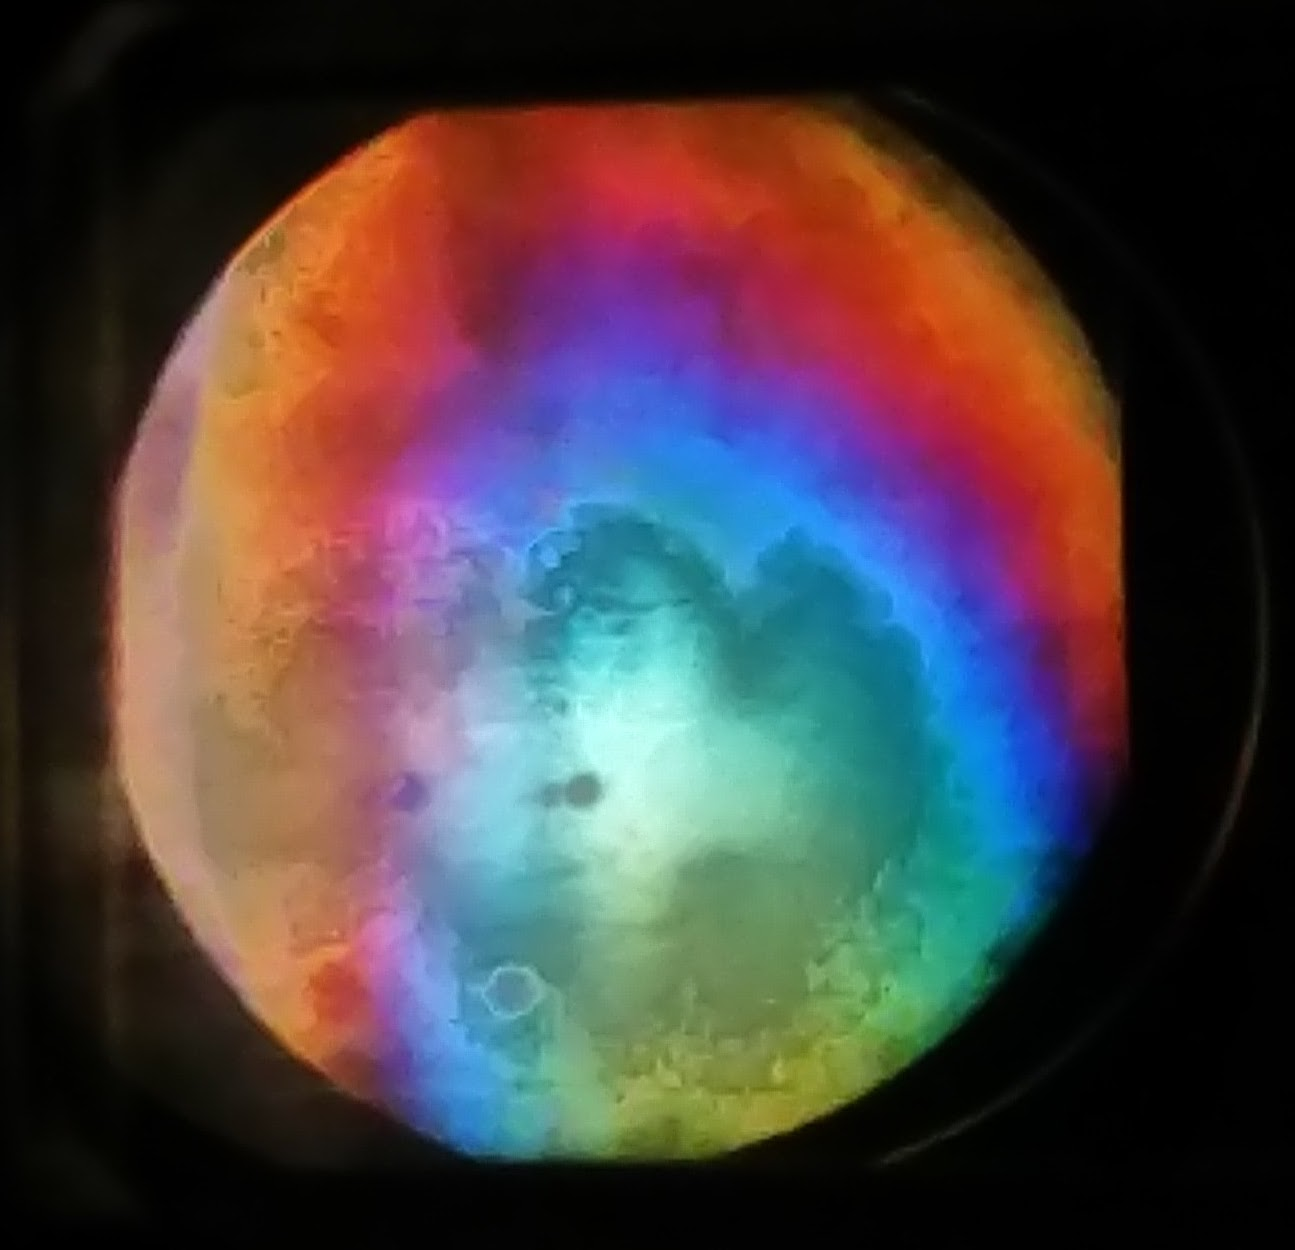
\includegraphics[width=0.7\textwidth]{./pictures/frange.jpg}
	\caption{frange di interferenza per luce bianca.}
	\label{fig:frangeb}
\end{figure}


Una ragione per cui il cammino ottico sui
de bracci dell'interferometro debba essere all'incirca uguale è
 il fatto che in tale configurazione l'interferenza non risulta
dipendente da $\lambda$: infatti con una sorgente così lontana
dall'essere monocromatica qualsiasi dipendenza significativa dalla
lunghezza d'onda risulterebbe nell'assenza di fenomeni apprezzabili a occhio nudo,
poiché le diverse componenti dello spettro della sorgente darebbero una distribuzione di frange
molto diversa, e la sovrapposizione di queste apparirebbe essenzialmente uniforme.